%!TEX root = ../report.tex

\section{Network Measurement}
Network performance can be measured for different metrics like throughput (bandwidth or packet rate), latency (average, median, standard deviation,\dots), frame loss rate, topology measurements or others with different circumstances (load, traffic type,\dots).
Different RFC standards exist as guideline.

\subsection{Throughput}
Throughput is usually limited by the line rate and the speed and size of the lookup tables.
It is measured in packets per second (not bandwidth) since routers usually only look at packet headers and not the entire packet, so the actual size has only a minor importance.
The worst case scenario regarding costs is network traffic at line rate and minimum packet size which is the minimum sized Ethernet packet plus the 7 byte preamble, 1 byte start-of-frame delimiter and the minimum inter-packet gap of 12 bytes, thus 84 bytes.\\
\vspace{4pt}

When testing, different measuring methodologies can be applied.
The simplest one is to apply the highest possible packet rate on A and measure the packet rate at B.
With this method, the devices might get overloaded though which leads to different behaviors.
So a better version is to apply varying rates on A and find the highest rate were no loss occurs (RFC 2544).
Problems of this approach again are that some devices loose packets when suddenly facing high packet rates due to energy saving mechanisms.
As a summary the best approach depends on the device under test.

\subsubsection*{Improving Throughput}
Potential bottlenecks for packet forwarding are CPU processing power, NIC processing power, Bus bandwidth, memory bandwidth or CPU caches.
As researches found out, the biggest limitation origins in the CPU.
The most time is spent to process, receive and transmit packets there.
When transferring the network stack from kernel to user space, performance can be significantly increased due to fewer expensive system calls, simplified memory management and batch processing through the whole application.
The disadvantages on the other hand are that only raw packets are handled, so protocols have to be reimplemented for every application, NICs can only be used by one application and there is no API compatibility to traditional user space applications.

\subsection{Parallel Packet Processing}
Modern NIC cards hare configurable to use multiple rx and tx queues to support multi-core parallelization to improve performance.
Several metrics to distribute incoming traffic on the queues exist:
\begin{itemize}
  \item Per-packet basis: Slow when protocol state has to be synchronized and might cause packet reordering
  \item Per-flow basis: Fast, protocols handled in the same core and cache and prevents packet reordering
  \item Explicitly: Useful for e.g. virtual machines, slower than flow-based though
\end{itemize}
Usually packet forwarding is done in kernel space due to better performance than the socket API.

\subsection{Latency}
Sources of latency are serialization, propagation and calculations where buffers usually are the biggest bottleneck.
Also the technique to receive packets plays a role:
\begin{itemize}
  \item one interrupt per packet: low latency but also low throughput because interrupts are expensive
  \item one interrupt for multiple packets: high throughput but also high latency
  \item no interrupts but polling based: low latency and high throughput but inefficient at low packet rates (busy waiting)
\end{itemize}

\subsection{Packet Generators}
Packet generators exist in hardware and software varieties.
Hardware generators are fast, precise and accurate.
Software ones run on cheap hardware and are very flexible but face challenges with rate control and time stamping.\\

To control the packet rate software implementations push single packets to the NIC where queues cannot be used.
Also the NICs work with asynchronous push-pull models which can lead to micro bursts and thus to unreliable, imprecise and bad performance.
Hardware generators on the other hand support hardware rate control where queues can be used and have good performance but they are quite inflexible.
To combine the advantages of both, one can disable hardware control and use invalid packets in the queues to control the rate since those are simply dropped by the device under test without much overhead.

\subsection{Internet Wide Scans}
When doing larger scale network scans are performed, several points have to be taken into consideration.
For one which targets are selected which might be a specific hitlist provided by e.g.\ traceroute, web server logs or traffic traces, certain IP addresses per subnet or even a full 0/0 scan.
Also there are performance requirements that need to be met and ethical considerations, too, since one causes sometimes large amounts of traffic on the scanned network.\\
\vspace{4pt}

\subsubsection*{Nmap}
Nmap is a common measurement tool which provides host discovery, service detection, OS detection and support for custom scripts.
It provides a multitude of scanning techniques:
\begin{itemize}
  \item TCP scan: Sends TCP packets with different flags set. A SYN scan checks for open ports, ACK scans scan for (un-) filtered ports by a firewall. Some more exist.
  \item ICMP scan: ping requests
  \item UDP payload scan: Sends UDP packets with different payloads
\end{itemize}
While scanning, randomization is used to avoid complaints of system administrators but only groups of 16k hosts are possible.
Nmap uses a stateful scanning approach to keep track of every packet in transit and to catch timeouts to try again to send packet.\\

\subsubsection*{Zmap}
A full Internet scan using nmap takes around 10 days which is quite slow.
For that reason, \textbf{zmap} was developed by the university of Michigan which is able to do a full scan in around 45 minutes.
It uses TCP SYN or UDP payload scans to find open ports and it is possible to distribute the scanning load on different machines and every IP is only scanned once.
The performance is reached by using raw sockets and not keeping state of packets which makes it impossible to detect timeouts though.
This is handled by cycling through the host IPs that have not jet responded a certain amount of times and then abort.
Furthermore without keeping states, incoming packets that belong to the scan are more difficult to identify.
Zmap therefore uses IP IDs which are used to generate a validation with AES which is stored in the packet sent e.g.\ in the sequence number
When receiving packets, they are validated using the validation, in the example from before $sequence~number- 1$.

\subsubsection*{IPv6 Scanning}
IPv6 scanning faces different challenges than IPv4 due to different routing, firewall and host configuration and the huge address space.
To to the amount of possible addresses it is not possible to do a 0/0 scan so hitlists are used to define the targets.
Sources for such hitlists are for example the Alexa Top 1 Million list (most popular websites), the Rapid7 DNS ANY list or DNS zone files (content of TLD name zones).
Also traceroute or passive sources like packet traces or flow data can be taken into account.\\
\vspace{4pt}

IPv6 scans can be evaluated for reachability or stability.
Also as long as the targets do not use IPv4 privacy extensions (Interface ID randomly chosen) the target device type can be determined.
The criterion is that routers usually have the IID ::1 for the default gateway.

\subsubsection*{Security Scans}
\textbf{TLS scans} are used to scan the state of TLS protocols like HTTPS or IMAPS in the Internet by analysing certificate chains, expiry and algorithms.
Scans are done by identifying hosts that offer TLS services, download the certificate chains and analise and validate these chains.\\
\vspace{4pt}

\textbf{SSH scans} mainly provide an overview over the security of the SSH configurations of hosts with public IPs.
Since SSH is mostly used for administrative or security sensitive contexts it is usually advisable to notify CERTs, watchlist services and blocklist operators about scans.
Also other measurements like an own scanning subnet with a abuse WHOIS email contact might be useful to hide one's identity.\\
In the past several internet wide SSH scans were performed which analysed key strength (length, debian weak keys, duplicate keys).\\
\vspace{4pt}

\textbf{IPMI (Intelligent Platform Management Interface)} is a out-of-band management system used in servers.
It uses a separate OS which has full access to the host OS\@.
IPMI scans try to detect known vulnerabilities in configurations, i.e.\ hosts should not be reachable from the public internet.
When combining IPMI responses with HTTPS reachability to detect IPMI web-interfaces which also might be vulnerable.
Compromised web servers again may lead to a compromised OS.\\
Internet wide scans for IPMI-over-IP devices are showing declining numbers of reachable devices.
Those who are reachable are heavily clustered in a view ASes though and detected HTTPS interfaces show that 90\% of them have 1024 bit or shorter keys.\\

\textbf{BACnet (Building Automation and Control Networks)} is a protocol that is used to control heaters, solar panels and other building automation aspects.
Access to those systems can lead to real world consequences.
It is based on UDP and has no build in security.
Devices providing this protocol have properties that can be queried via a SingleProperty or MultipleProperty request which enables attackers to generate larger responses which results in easier DOS attacks.
To detect these easily possible attacks, scans are performed to check the BACnet deployment in the internet.

\subsubsection*{Ethical considerations}
It is usually advisable to take some ethical steps before doing Internet wide scans.
These include reducing the intrusiveness of scanning by avoiding logins or limit the scanning rate, providing information on the scanning machine's website, respond quickly to every inquiry and abuse email and offer possibilities for blacklisting IPs.
A general guideline here is to be the "nice guy".

\subsection{Passive Measurements}
Passive network measurement does not cause additional traffic like the approaches mentioned above but uses monitoring probes to analyze existing traffic.
Important metrics here are traffic volume, traffic composition and packet inter-arrival times with different levels of granularity.
When captured, different analyses can be performed, e.g.\ network utilization, QoS parameters, detection of failures and anomalies or traffic characterization.
These informations might be useful for accounting, security or traffic engineering.\\

The capturing hardware usually has to be able to perform on multi-gigabit/s links with relative cheap costs and simple deployment.
Common approaches to these requirements are high-end network adapters with large amount of memory and functionality (still cheap?), sophisticated algorithms by eliminating copying of packets amongst others, sampling (probabilistic filtering of packets), filtering (mask, router state, hash based) and aggregation.\\

The process passive measurement is depicted in Figure~\ref{fig:passive_network_measurement}.
\begin{figure}[h]
  \centering
  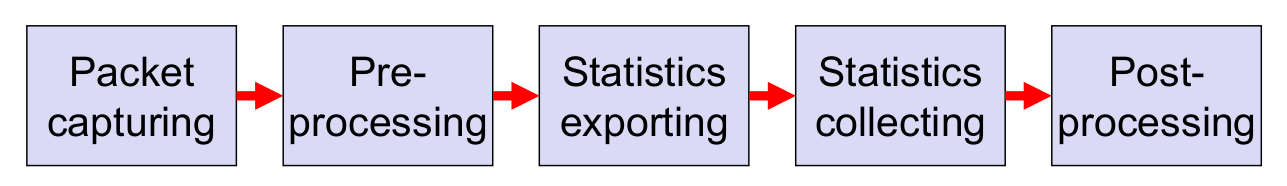
\includegraphics[width=.8\textwidth]{figures/passive_network_measurement.png}
  \caption{Passive Network Measurement Process}\label{fig:passive_network_measurement}
\end{figure}

\textbf{Packet capturing} is assisted by hardware.
Server NICs have direct access to the main memory without processor support and do batch processing to reduce copy operations.
Also special monitoring interface cards exist which usually only are able to receive data and provide certain processing features like filtering, high-precision time-stamps and others.

\subsection*{Flow-based Traffic Measurements}
Flows describe packets which belong together like all packets of a TCP connection (IP-5-Tuple).
Flow data is usually measured passively on the network and is exported when on of two timeouts runs out.
The inactive timeout starts at the last received packet of a flow and is reset with every packet.
The active timeout starts with the first packet of a flow and is only reset if it expires.
The inactive timeout was designed to export flow data of short lived flows whereas the active timeout sends data during a flow is active for long lived ones.

\subsubsection*{IP Flow Information eXport (IPFIX)}
The IPFIX protocol was defined by the IETF in RFCs and is an extensible flow exportation protocol.
The extensibility is achieved by differentiating between template and data records where the template defines the data format for the data records.\\
During measurement, statistical counters and values are updated and whenever a flow terminates, the data is exported via SCTP or, if available, TCP or UDP.\\
The metering process of IPFIX includes packet header capturing, timestamping, classifying and the maintaining of flow records where a flow record contains information about measured properties of the flow like total number of bytes in the flow or IP addresses.
Exporting then sends flows to one or more collecting processes.
In the end data is collected from all capturing points and further processed.\\
Metering and exporting can be done on network devices directly, or be on separate hardware.
Collecting is usually done separately.\\
Sampling and filtering can be used for very high-speed networks.

\subsubsection*{Anomaly Detection with Machine Learning}
Machine Learning can be used to detect anomalies based on flow data.
For this, feature vectors have to be created from flow data with numerical and categorical semantics.
An example for such a transformation of the data is shown in Figure~\ref{fig:ml_feature_vector_creation}.
\begin{figure}[h]
  \centering
  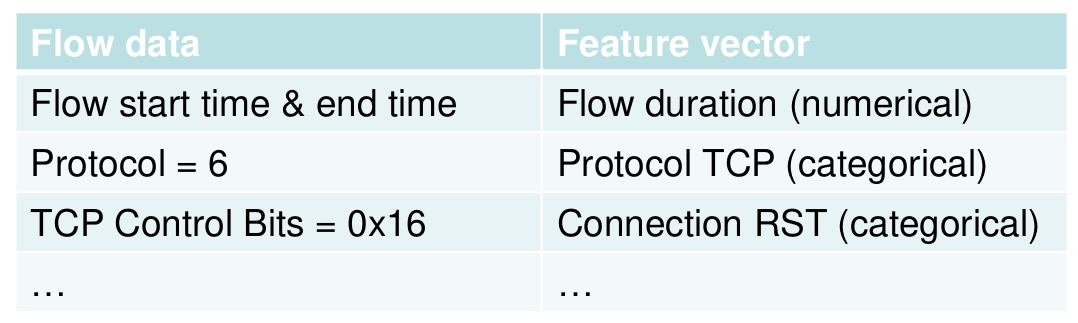
\includegraphics[width=.7\textwidth]{figures/ml_feature_vector_creation}.
  \caption{Feature Vector Creation}\label{fig:ml_feature_vector_creation}
\end{figure}

\textbf{Supervised machine learning} then uses labeled training data to learn what is benign and malicious traffic.
\textbf{Unsupervised ML} on the other hand has no training data available.
It tries to find clustered data and outliers.
The outliers then represent an anomaly.\\

To assess the quality of these approaches, different metrics can be used:
\begin{itemize}
  \item Precision = $\frac{\text{true positives}}{\text{true positives + false postives}}$\\
    How many of the detected anomalies are actual anomalies?
  \item Recall = $\frac{\text{true positives}}{\text{true positives + false negatives}}$\\
    How many of all actual anomalies did I detect as anomalies?
  \item Accuracy = $\frac{\text{true positives + true negatives}}{\text{all}}$\\
    How many positive and negative classifications are correct?
\end{itemize}
The goal is to decrease false positives and negatives here, but in reality decreasing on type of error increases the other.

\subsection{Amplification Attack Detection}
In amplification attacks, the attacker sends small request to an amplifier network with a spoofed IP address which generate large response packets to the victim (owner of the spoofed address).\\
The amplifier network might be able to detect such an attack though by passively measuring incoming and (potential) outgoing traffic.
Different characteristics can be used then to identify an attack:
\begin{itemize}
  \item Amplification factor: compare incoming and outgoing traffic, if asymmetric an attack is possible
  \item Packet size similarity: Same sized packets incoming frequently
  \item Payload similarities: Packets from the attacker have similar payload content. Payload similarities are detected by a low entropy.
  \item Unsolicited ICMP messages: backscatter ICMP message of the victim are indicator for an attack
  \item TTL measurements: path form attacker $\neq$ path from amplifier to victim indicates an attack
\end{itemize}

\subsection{Hybrid Measurements}
A hybrid approach between active and passive measurement can be taken where packet flows are modified by piggybacking or header modification.
This enables adding additional information to packets without applying additional load to the network.
This has to be taken with care though, since people might not like this.

\subsection{Detecting Traffic Misdirection in Interdomain Routing}
\begin{figure}[H]
  \centering
  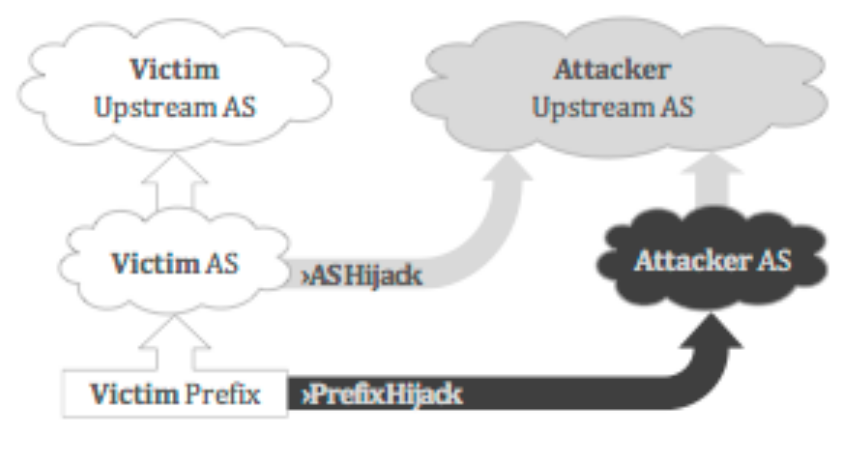
\includegraphics[width=.6\textwidth]{figures/as_and_prefix_hijacking.png}
  \caption{Possible attacks}\label{fig:fig:as_and_prefix_hijacking}
\end{figure}

In prefix hijacking attackers announce a victim's (sub-) prefix to other ASes.
We already have real-time detection for that.
AS Hijacking is a more sophisticated approach where a letter of authorization has to be accepted by ISPs as a legitimation to advertise resources of a customer's AS\@.
Such an attack is usually carried out over several month.
In the example of LinkTel, the attackers re-registered an expiring domain (link-telecom.biz), forged an letter of authorization to the upstream provider and announced false BGP routes.\\
In 2013 an escalation warning system for AS hijacking was designed at the TUM which uses passive monitoring of DNS expiry an re-registration and analysis of reverse DNS and BGP activity to identify vulnerable targets.

Current hijack detection is done via multiple traceroute scans from multiple vantage points.
To identify the poisoned part of the network, last hops to the target prefix and downstream graph of last hops are regarded.
Possible detection metrics are a detection of an odd distribution of first-rank countries (5 neighbours Germany, 1 New Zealand), an odd distribution of first-rank ASes or odd RTTs.
Also Exclusive AS connectivity can be used to detect how many ASes in the graph are connected exclusively through one neighbour of the target.
With that approach a segmentation of the graph is possible which allows the specification of the impact of a possible hack.\\
